\section{Method}
This section explains how the implementation was done and how the experiments were conducted. After that follows an outline of the experiment setup and a motivation for the designs of the experiments.
\subsection{Implementation}
The implemented word predictor had three basic components: N-grams with probability smoothing, grammar constraints and context recognition. The implementation was done using two NLP-libraries and several books to make a corpus. KYLM\footnote{A full list of resources can be found in section \ref{sec:resources}} was a library capable of producing N-grams with different smoothing techniques. We used it to process our corpus and make an ARPA-file, consisting of N-grams of different sizes and their probability derived from the corpus and chosen smoothing technique. We also used OpenNLP for part-of-speech-tagging that was used in the implementation of grammar constraints in the word predictor. The rest of the program: searching the ARPA-files, grammar constraints, context recognition and user interface was implemented by the authors.

To test our hypotheses, a qualitative inductive method was used. Evaluation and comparison of the different functionalities was made by measuring keystroke counts. This was a widely used method\cite{keystrokes}, and suited our project as it is an objective performance evaluation, and user interface/experience was of no interest to the study.

In a keystroke count experiment, for a given word, the number of keystrokes are the number of keys that the participant has to press in order for the word predictor to suggest the word the participant meant to write. In this experiment, given previous words, the word predictor may be able to suggest the thought of word without any strokes in which case the keystroke count for that word is zero. Spaces between words did not count as keystrokes.

\subsection{Evaluation}

\begin{figure}[t]
\center
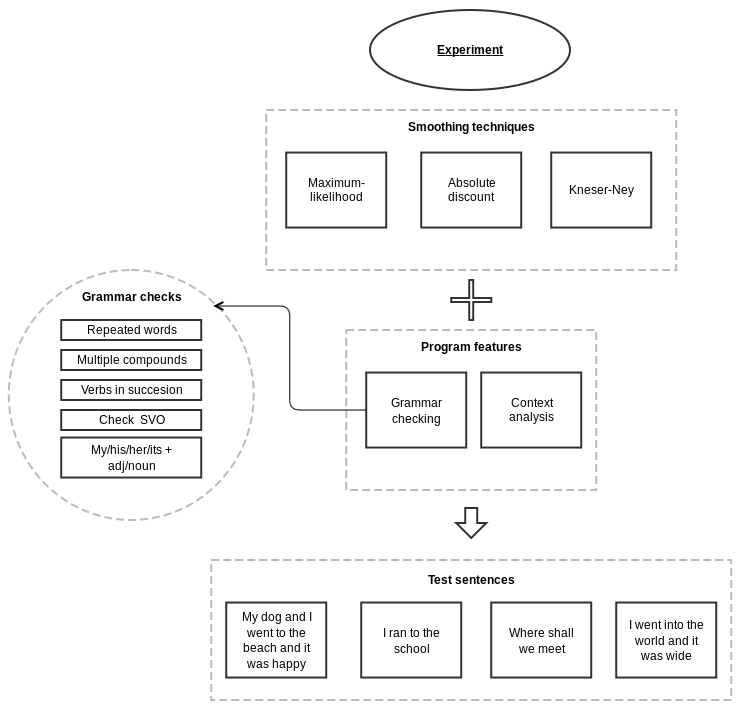
\includegraphics[width=0.7\textwidth]{img/experiment_diagram.png}
\caption{Diagram showing how experiments were generated}
\label{fig:experiments}
\end{figure}

The process of generating experiments is shown in figure \ref{fig:experiments}. Four sentences that were thought to bring out the differences in the different functionalities were constructed. Tests were then performed for each sentence, for each combination of functionalities and for each smoothing technique, which made a total of 48 different tests. After that, some tests were rerun with case-insensitivity. OpenNLP did not work well with case insensitivity. For the reruns, grammar constraints were therefore always set to \emph{off}, resulting in an additional 24 tests.

\subsubsection{Experimental setup}
\paragraph{Corpus}
The corpus used in the experiments consisted of 10 books\footnote{The full list of books can be found in section \ref{sec:resources}} of varying themes and content, downloaded from \url{http://www.gutenberg.org/}. Choosing the books was done at random but from different categories such as children's books, science fiction and philosophy.

The corpus was manipulated by removing citation marks, underscores and new lines. Periods, commas and question marks were made into separate words by adding a space before them.

The reasoning for first using a case-sensitive corpus was that the POS tagging required for grammar constraints was case-sensitive. However, after our first test round it was clear that the grammar constraints did not help much. A lowercase corpus was considered to produce better probabilities since there is no differentiating between the start of a sentence and the start of a bi-sentence. Therefore another corpus was created where all words were converted to lowercase to see if more keystrokes could be saved, even though this corpus could not be used together with grammar constraints.